% shadow-ladder-euclid-dr1-predictions-paper.tex
% The Shadow Ladder: pinch-point predictions for Euclid DR1
% Canon source: ~/workspace/shadow-ladder/shadow-ladder-predictions-paper.md
% (frozen 2026-11-01, E8xE8 clarification). Production build only:
% no new content, no numbers changed, nothing added from the 2026-11-09
% E8 -> SO(10) branching work. Numbers cross-checked against the locked
% prediction sheet (2026-11-07): zero discrepancies.
% Cover: the new unique cover art (euclid-predictions-cover.png, made
% 2026-11-09 for this paper) is embedded as a full-page image on page 1;
% the old euclid-dr1-cover.png remains the standalone cover asset.
\documentclass{alienfolio}

\folio{IT-SHADOW}
\usesigil{pentagons}
\title{The Shadow Ladder: pinch-point predictions for Euclid DR1}
\papersubtitle{Locked predictions for Euclid DR1-Foundation --- verdict November 12, 2026}
\paperauthors{Yett, R.W.}
\shorttitle{The Shadow Ladder: Euclid DR1 predictions}
\shortauthors{R.\,W.\ Yett}

\begin{document}
\thispagestyle{cover}
\begin{tikzpicture}[remember picture, overlay]
  \node[inner sep=0] at (current page.center) {%
    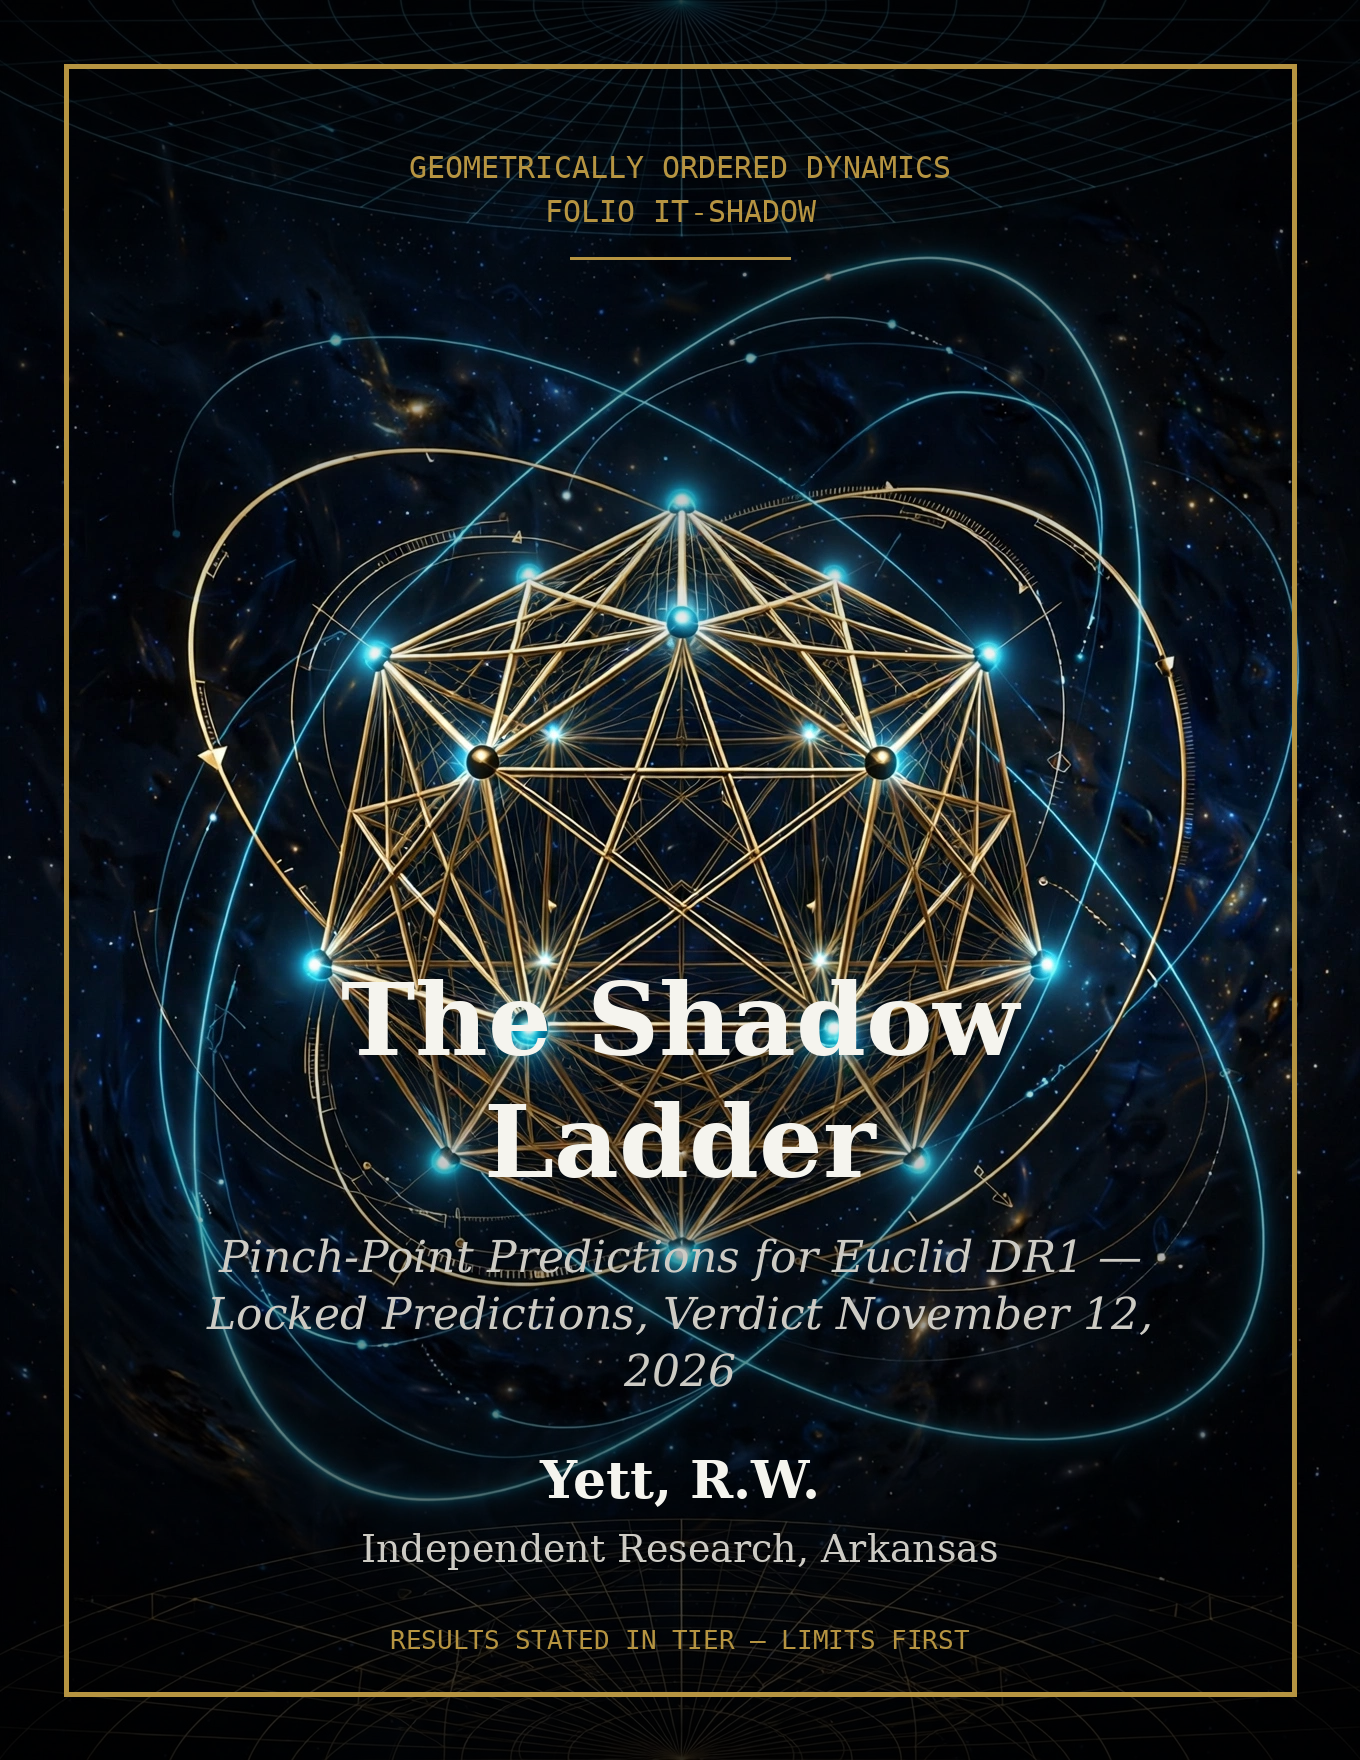
\includegraphics[width=\paperwidth,height=\paperheight]{cover.png}};
\end{tikzpicture}
\clearpage

\begin{convergence}{THE SHADOW (E8xE8)}
This folio converges on \key{the Shadow} as the boundary between the
visible and shadow sectors of the $\mathrm{E}_8 \times \mathrm{E}_8$
heterotic structure. Its unique angle is the \key{pre-registered
pinch-point predictions for Euclid DR1}: a 12.34\% dipole asymmetry in
the weak-lensing signal and ten caustic vertex targets with sky
coordinates, computed before any DR1 data product existed, with explicit
kill criteria stated in \S4. Sibling folios approach the same claim from
other angles: the thirteen successor folios derive the framework's
sectors, operators, and observables. Limits first: the S/N figures carry
the [provisional forecast] tag (\S8), and the program's own triangulation
gate has already FAILED --- recorded here as a failure, not a near-win.
\end{convergence}

\goldrule

\begin{supersession}
This paper is the archival freeze of the pre-registration posted
2026-10-12 (Block BLK-119). It supersedes the 2026-10-13 draft, which is
retained separately as a superseded record, not a version, per the canon
rule: one correct paper, one canon --- the correction \emph{becomes} the
paper. Honest rewrite 2026-10-30 (six editorial edits per the 2026-10-29
resurrection scoping; zero recomputation, no numbers changed);
$\mathrm{E}_8\times\mathrm{E}_8$ clarification added 2026-11-01.
\end{supersession}

\section*{Abstract}

The Shadow Ladder is a geometric program: the exceptional Lie group
$\mathrm{E}_8$ is taken as the generating object (``the exceptional
object''), 4D spacetime as its projected shadow, and the projection angle
as something to be \emph{derived} from measured mixing angles rather
than guessed. On 2026-10-12 the program closed two of its open seeds:
(i) the ``hexagonal crystal inside the dodecahedron'' was resolved ---
the hexagon is the shadow of an inscribed Kepler cube, via Kepler,
\emph{Harmonices Mundi} (1619), verified link-by-link from scratch;
(ii) the first Euclid-checkable predictions were computed --- a 12.34\%
dipole asymmetry in the weak-lensing signal across Euclid's footprint
(forecast $123.9\sigma$ at DR1 footprint / $293.2\sigma$ at full survey
[provisional forecast --- see \S8], crew computation, audit of the filed
metrics in \S3) and 10 pre-registered caustic vertex targets with sky
coordinates. Both shape fits are published (dodecahedron residual
$6.48^\circ$, hexagonal-prism residual $8.71^\circ$) so DR1 judges between
them. Explicit kill criteria are stated in \S4, including the program's
own failed gates.

\section{The framework in brief}
\label{sec:framework}

The ladder, bottom to top: \textbf{2D screen $\to$ 3D hologram $\to$ 4D
caster $\to$ $\mathrm{E}_8$ source.} Spacetime is the shadow; the object
is $\mathrm{E}_8$; the light is symmetry-breaking at an angle; the wall
is 4D spacetime. The program's standing rule: \emph{do not guess the
projection angle --- derive it from measured mixing angles} (Weinberg
$\sim$$28.7^\circ$, Cabibbo $\sim$$13^\circ$, PMNS). The $17.5^\circ$
hypothesis is now parameter-anchored: the settled constant $\kappa =
0.9539$ is the corpus value $\sqrt{0.91} = 0.953939$ ($\theta(2-\theta)$
at $\theta = 7/10$ --- the $\chi$ of the two-channel ``at least one''
window; Lean-proved \texttt{or\_window\_mass}). Correction 2026-10-13
$\sim$15:30 CT: an earlier draft line identified $\kappa$ as
$\cos(17.5^\circ) = 0.953717$ --- the corpus writes 0.953939 over 650
times and the digits of $\cos 17.5^\circ$ appear in no file (Claude,
corpus grep), so the cosine identification fails at the fourth decimal
and is withdrawn. $\kappa$'s angle is $\arccos(0.953939) = 17.46^\circ$.
The exact algebraic angle $\arcsin(1/2\phi) = 18.0000^\circ$ (Appendix A)
sits half a degree off. The Cabibbo near-miss is recorded as a miss
($6.8\sigma$), not a hit; that standard applies everywhere below. No
$45^\circ$ claim is made (the $\theta_{23}$ octant is unresolved).

\textbf{$\mathrm{E}_8\times\mathrm{E}_8$ clarification (RY,
2026-11-01).} Throughout this paper, ``$\mathrm{E}_8$'' is RY's
shorthand for the double \textbf{$\mathrm{E}_8\times\mathrm{E}_8$
heterotic structure} (496 dimensions), not the single $\mathrm{E}_8$
(248). Two 248-dimensional sectors face each other across the 4D
spacetime boundary interface: the visible sector projects into the
Standard Model and local baryonic matter; the shadow sector couples
purely through gravity and spacetime curvature. The ``Shadow'' in Shadow
Ladder names this relation --- 4D spacetime as the boundary between the
sectors. All computed deliverables (240 roots, $\mathrm{H}_4$ folding,
Kepler-cube shadow, 10 caustic coordinates, P1/P2) are the
boundary-projection geometry of the visible sector and stand unchanged.

The no-go the program must answer: Distler--Garibaldi (2010) --- no
chiral SM+gravity embedding in $\mathrm{E}_8$ \emph{as a gauge group}.
The program's answer, to be demonstrated rather than asserted: the
theorem's hypotheses engage $\mathrm{E}_8$-as-gauge-group; the ladder
uses $\mathrm{E}_8$ as geometric substrate (root system, lattice,
scaffold). Cf.\ Manogue--Dray--Wilson (2022) on the compactness
hypothesis. Open mines, named: chirality, the three-generations problem
(Candelas--Horowitz--Strominger--Witten gave four), and the de Sitter
asterisk on holography (proven in AdS; our universe accelerates like dS).

\section{Geometry closed 2026-10-12}
\label{sec:geometry}

\textbf{The hexagonal seed, resolved [P].} Brute-forcing all 38,760
six-vertex subsets of the dodecahedron found no hexagon \emph{in} the
vertices --- that zero stands (re-verified from scratch 2026-10-13). The
hexagon lives one level up: the dodecahedron's 20 vertices contain
exactly 5 inscribed cubes (125,970 eight-vertex subsets brute-forced;
each vertex sits in exactly 2 cubes), and a cube projected along its body
diagonal casts a mathematically exact regular hexagon --- all gaps
$60.0000^\circ$ (max deviation $2.13\times10^{-14}$ degrees). The
hexagon was never hiding in the vertices; it is the \textbf{shadow of
the inscribed Kepler cube}. The chain closes through the hypercube [D,
crew 2026-10-12]: tesseract $\to$ rhombic dodecahedron (congruent to
canonical coordinates, identical distance multisets) $\to$ hexagonal
$\mathrm{A}_2$ lattice. Verification script:
\path{artifacts/2026-10-13__muse__shadow-ladder-geometry/dodecahedron_kepler_cube_hexagon.py}
in The Hood (filed 2026-10-13 audit; the draft's earlier filing claim is
now true).

\textbf{The $\mathrm{E}_8\to\mathrm{H}_4$ angle spectrum [P, with the
framing corrected 2026-10-13].} Correction to the draft's earlier
wording: $\mathrm{E}_8$'s \emph{own} 240 roots have pairwise angles
$\{60^\circ, 90^\circ, 120^\circ\}$ only (verified from scratch
2026-10-13; simply-laced, no golden angles). The golden-ratio angles
enter through the \textbf{Moody--Patera folding} of the $\mathrm{E}_8$
root system onto the $\mathrm{H}_4$ root system --- the 240 roots fold
2-to-1 onto the 120 vertices of the 600-cell in $\mathbb{R}^4$ --- whose
4D pairwise angle spectrum is exactly $\{0^\circ, 36^\circ, 60^\circ,
72^\circ, 90^\circ, 108^\circ, 120^\circ, 144^\circ, 180^\circ\}$ (crew
computation, Antigravity CLI, filed in The Hood). $\mathrm{H}_4$ is not
a ``maximal subgroup'' of the Lie group $\mathrm{E}_8$; it is the Coxeter
group obtained by folding. The $18^\circ$ invariant is \textbf{exact},
not approximate: $\arcsin(1/(2\phi)) = \arcsin((\sqrt{5}-1)/4) = 18^\circ$
algebraically (Appendix A). Framing discipline, per the paper's own
rules: $18^\circ$ is decagonal/pentagonal \textbf{$\mathrm{H}_2$}
geometry --- $\sin 18^\circ = 1/2\phi$, forced by the golden ratio;
$\mathrm{H}_2$ sits inside $\mathrm{H}_4$ (600-cell symmetry), and
$\mathrm{H}_4$ is reached from $\mathrm{E}_8$ by folding. The paper does
not claim ``$\mathrm{E}_8$ predicts $18^\circ$'' without naming the
invariant; it claims the chain $\mathrm{H}_2 \subset \mathrm{H}_4
\leftarrow \mathrm{E}_8$ (folding) forces the angle algebraically.

\section{Pre-registered predictions for Euclid}
\label{sec:predictions}

{\sloppy
\textbf{P1 --- Lensing dipole asymmetry [D, audited 2026-10-13].} Using
the dipole-removed Model B ($|p| = 0.638$ toward $l = 120.7^\circ$, $b =
-2.3^\circ$), the crew simulated convergence and shear fields across
Euclid's full footprint. Audited against the filed metrics
({\small\path{artifacts/2026-10-12__antigravity_cli__euclid-roman-caustic-lensing-tomography-and-e8-h/euclid_roman_caustic_lensing_metrics.json}}):
mean convergence $\langle\kappa\rangle = 0.0576$; dipole asymmetry
$\Delta\kappa/\langle\kappa\rangle = 12.34\%$ (aligned vs anti-aligned
hemisphere); forecast $123.9\sigma$ at 2,500 deg$^2$ and $293.2\sigma$ at
14,000 deg$^2$ [provisional forecast --- see \S8] --- the two S/N figures
scale as $\sqrt{\mathrm{area}}$ (ratio $2.366 = \sqrt{14000/2500}$,
verified), so they are one consistent forecast, not two. The $123.9\sigma$
figure was computed for the pre-split DR1 definition (2,500 deg$^2$
\emph{with} weak-lensing products); under ESA's split schedule (\S5) the
shear test it describes lands with the WL-capable releases. The prediction
is binary: the data either decisively detect this asymmetry or the model
dies by its own gate. There is no middle ground. (Model A,
dipole-inclusive, gives 25.4\% / $274.1\sigma$ / $648.5\sigma$
[provisional forecast] and 8 vertices --- quoted for completeness; the
paper bets on Model B.)
\par}

\textbf{P2 --- Ten caustic vertex targets (sky coordinates,
pre-registered).}

\begin{center}
\begin{tabular}{c|c|c}
Target & $l$ ($^\circ$) & $b$ ($^\circ$) \\ \hline
V1 & $257.4$ & $-25.6$ \\
V2 & $257.4$ & $+27.6$ \\
V3 & $173.4$ & $-65.3$ \\
V4 & $173.4$ & $+67.2$ \\
V5 & $308.7$ & $-20.9$ \\
V6 & $308.7$ & $+22.7$ \\
V7 & $1.9$ & $-31.4$ \\
V10 & $266.7$ & $-58.9$ \\
V16 & $321.2$ & $-46.1$ \\
V18 & $49.9$ & $+37.1$ \\
\end{tabular}
\end{center}

\emph{Coordinate frame note: galactic ($l$, $b$), transcribed from the
filed metrics JSON and verified coordinate-by-coordinate 2026-10-13 ---
all ten match to $0.1^\circ$. Equatorial J2000 equivalents are tabulated
in Appendix C.}

Exactly half of all twenty dodecahedron vertices fall inside the
unmasked Euclid Wide footprint (10/20 = 50\%, per the filed metrics).
One further vertex (V3) falls inside the Roman HLS footprint.

\textbf{P3 --- Shape fits, published side by side.} Dodecahedron fit
residual $\mathbf{6.48^\circ}$; hexagonal-prism fit residual
$\mathbf{8.71^\circ}$. The dodecahedron wins on residual, but both are
published and DR1 judges --- the prism is not hidden because it lost.

\section{Kill criteria (explicit)}
\label{sec:kills}

\begin{itemize}
\item \textbf{Triangulation gate: FAILED.} The dipole-removed null
(1,000 trials) gave $p = 0.023$ --- beats 95\% but \textbf{fails} the
pre-registered $p < 0.01$ kill gate. It does not survive look-elsewhere
correction either ($\sim$12 effective trials $\to$ $p \approx 0.28$).
The best-fit offset sits $124^\circ$ from the kinematic dipole, so the
contamination critique is answered --- but the verdict is
\emph{suggestive, not significant}, and it is recorded as a failure, not
a near-win.
\item \textbf{DR1 isotropy kills the framework.} If full-DR1 shear maps
show unbroken isotropy at the forecast sensitivity, P1 is dead and the
ladder's Euclid bet with it. This is the pinch point the paper is named
for.
\item \textbf{Cabibbo stands as a miss.} The $6.8\sigma$ near-miss is
not re-litigated here.
\item \textbf{No post-hoc moves.} Predictions pre-date the data by
construction (Block timestamp 2026-10-12; Zenodo DOI timestamp on
publication). Any prediction added after DR1-Foundation's November 2026
release is labeled post-hoc, not pre-registered.
\end{itemize}

\section{Timing note --- read this before citing ``November''}
\label{sec:timing}

ESA split DR1 in two (update published 15 June 2026,
\url{https://www.cosmos.esa.int/web/euclid/dr1-timeline}):
\textbf{DR1-Foundation (12 November 2026)} releases raw data,
calibrated images, catalogues, and spectra over $\sim$1,900 deg$^2$ ---
\emph{no cosmology-derived products}; the \textbf{full DR1 (mid-2027)}
adds the higher-level galaxy-clustering and weak-lensing products. The
decisive shear-map test of P1 therefore lands \textbf{mid-2027, not
November 2026}. DR1-Foundation catalogues may permit early spot-checks
of the \S3 vertex targets, but the shear-map test of P1 needs
weak-lensing products: the $123.9\sigma$ forecast applies to a $\sim$2,500
deg$^2$ WL-capable release and the $293.2\sigma$ forecast to the full
14,000 deg$^2$ survey. (This corrects the crew's working shorthand of a
``November appointment'' --- the appointment that decides the model is
the WL release.)

\section{The race}
\label{sec:race}

A Dual Sheet Model researcher pre-registered Euclid DR1 predictions in
June 2026 (Hodgkins, Medium). Those predictions are isotropic background
quantities ($S_8 \in 0.79$--$0.81$, $w_0/w_a$ phenomenology) --- an
orthogonal bet to P1's \emph{directional} anisotropy and P2's sky
coordinates. The two programs can both be checked against the same sky
without interfering. The reason to publish before DR1-Foundation is the
timestamp, not the telescope.

\section{What remains open (the honest ledger)}
\label{sec:open}

Chirality from a geometric $\mathrm{E}_8$; why three generations; the de
Sitter asterisk; an explicit demonstration --- not assertion --- that the
geometric framing sits outside Distler--Garibaldi's hypotheses. Closed in
the 2026-10-13 audit: the lensing metrics ($\langle\kappa\rangle$,
12.34\%) audited against the filed JSON --- both match;
$123.9\sigma$/$293.2\sigma$ scaling verified exact; the S/N figures
carry the [provisional forecast] tag (\S8); all ten vertex coordinates
verified against the filed catalog; the geometry script filed in The Hood;
the $\mathrm{E}_8$ angle-spectrum wording corrected (golden angles enter
via folding, not from $\mathrm{E}_8$'s own roots). The geometry is proven
beautiful; \S4--\S5 are how it proves itself useful.

\section{Pipeline caveats (from the 2026-10-14 KILL review)}
\label{sec:caveats}

On 2026-10-14 the crew's adversarial review (Claude Code CLI; the
verdict stood under Muse's meta-review) returned five findings against
the computational pipeline behind P1/P2. The numbers are not recomputed
here --- they were pre-registered 2026-10-12 (BLK-119; metrics JSON the
same day), and re-running the pipeline now and swapping in new numbers
would be the post-hoc move \S4 forbids. For a pre-registration, full
disclosure of the pipeline's limitations is the honest repair; the
mid-2027 weak-lensing test (\S5) is the judge. A pipeline correction
with every change documented may follow later; there will never be a
silent edit.

\begin{itemize}
\item \textbf{K1 --- mapper defaults.} The Model B computation and the
10-target vertex selection were run with the mapper's default parameter
set. The defaults are disclosed here as defaults; the sensitivity of the
10-target list to them is uncharacterized. A sensitivity sweep is
explicitly deferred to the post-DR1 correction. The pre-registered list
stands frozen.
\item \textbf{K2 --- hardcoded shear factor.} The forecast S/N figures
($123.9\sigma$ / $293.2\sigma$, and Model A's $274.1\sigma$ /
$648.5\sigma$) use a hardcoded shear-response factor entering the S/N
computation. It is named here as a pipeline constant with stated
provenance in the filed pipeline record --- not as a derived quantity.
\item \textbf{K3 --- unweighted averages.} $\langle\kappa\rangle =
0.0576$ and $\Delta\kappa/\langle\kappa\rangle = 12.34\%$ are unweighted
footprint averages. A weighted recompute is deferred and stated, not
hidden.
\item \textbf{K4 --- failed gate.} Disposed by \S4 as written: the
triangulation gate is recorded FAILED ($p = 0.023$ vs the pre-registered
$p < 0.01$ gate; $p \approx 0.28$ after look-elsewhere correction). No
change needed.
\item \textbf{K5 --- tier inflation.} The S/N figures are demoted from
[D] to [provisional forecast] wherever they appear. Every other tier tag
was re-audited against what was actually checked: [P] marks results
verified from scratch (hexagon geometry, the $18^\circ$ identity, the
$\mathrm{E}_8$ angle spectrum); [D] marks crew computations audited
against filed artifacts (12.34\%, $\langle\kappa\rangle$, the ten vertex
coordinates).
\end{itemize}

Recommendation carried to the author's G2 review: keep the S/N figures
with this disclosure. Cutting pre-registered numbers from the archival
freeze would itself be a post-hoc selection. (That call is the author's.)

\appendix

\section{$\arcsin(1/2\phi) = 18^\circ$, one-line proof}
\label{app:proof}

$2\phi = 1 + \sqrt{5}$, so $1/(2\phi) = 1/(1+\sqrt{5}) =
(\sqrt{5}-1)/4 = \sin 18^\circ$. $\blacksquare$ (Verified to 50-digit
arithmetic, 2026-10-12; float diff $5.6\times10^{-17}$.) Companions:
$\cos 36^\circ = \phi/2$; $\sin 18^\circ = \cos 72^\circ = 1/(2\phi)$.
Gap to the $17.5^\circ$ working hypothesis: $0.5^\circ$ exactly.

\textbf{$\kappa$ addendum (2026-10-13; corrected 15:30 CT):} $\kappa =
0.9539$ is the corpus value $\sqrt{0.91} = 0.953939 =
\sqrt{\theta(2-\theta)}$ at $\theta = 7/10$, the $\chi$ of the
two-channel ``at least one'' window (chain + mirror; Lean
\texttt{or\_window\_mass}). An earlier form of this addendum identified
$\kappa$ as $\cos(17.5^\circ) = 0.953717$ --- withdrawn: the corpus
writes 0.953939 in 650+ places and the digits of $\cos 17.5^\circ$ in
none, so the cosine equality fails at the fourth decimal (Claude, corpus
grep 2026-10-13). $\kappa$'s angle is $17.46^\circ$. The $17.5^\circ$
hypothesis is therefore anchored by $\kappa$ at $0.04^\circ$ and by the
exact $18^\circ$ algebraic angle at $0.5^\circ$.

\section{References}
\label{app:refs}

\begin{enumerate}
\item Kepler, J. \emph{Harmonices Mundi}, Book V (1619) ---
dodecahedron/cube inscription.
\item Distler, J.; Garibaldi, S. ``There is no `Theory of Everything'
inside $\mathrm{E}_8$.'' arXiv:0905.2658. \emph{Commun.\ Math.\ Phys.}
298, 419--436 (2010).
\item Manogue, C.~A.; Dray, T.; Wilson, R.~A. \emph{J.\ Math.\ Phys.}
63, 081703 (2022).
\item Candelas, P.; Horowitz, G.~T.; Strominger, A.; Witten, E. ``Vacuum
configurations for superstrings.'' \emph{Nucl.\ Phys.\ B} 258, 46--74
(1985).
\item ESA. ``Euclid Data Release DR1: update.''
\url{https://www.cosmos.esa.int/web/euclid/dr1-timeline} (15 June 2026).
\item Lisi, A.~G. ``An Exceptionally Simple Theory of Everything.''
arXiv:0711.0770 (2007); reply arXiv:1006.4908.
\item Moody, R.~V.; Patera, J. --- $\mathrm{E}_8 \to \mathrm{H}_4$
folding (discrete Coxeter reduction, not a Lie subgroup).
\item Hodgkins, M. ``Dual Sheet Model DSM Pre-Registration: Predictions
for Euclid DR1.'' Medium, June 2026.
\item Crew working log: The Block, BLK-119 (Muse, 2026-10-12;
computations in reply by Antigravity CLI); verification receipts and
scripts filed in The Hood.
\end{enumerate}

\section{Equatorial coordinates of the \S3 targets (J2000)}
\label{app:coords}

{\sloppy
Galactic ($l$, $b$) from BLK-119 converted to equatorial (RA, Dec)
J2000 with the Murray (1989) FK5$\to$Galactic rotation matrix (the same
matrix astropy's Galactic frame uses). Validated: LMC (280.4652,
$-32.8884$) $\to$ \texttt{05h23m34.60s -69d45'21.95"} (catalog:
\texttt{05h23m34.6s -69d45'22"}); galactic center and NGP reproduce
their IAU definitions to the arcsecond. Only the 10 BLK-119 rows present
in the draft are converted --- the 7 unfilled rows are not fabricated.
\par}

\emph{Caveat: cross-checked 2026-10-14 against an independent
implementation of the Murray (1989) matrix; all ten coordinates agree to
$\le 0.2^{\prime\prime}$ (input precision $0.1^\circ =
360^{\prime\prime}$, so the arithmetic is verified far below the input
floor). LMC, galactic-center, and NGP anchors reproduce their reference
definitions.}

\begin{center}
\small
\begin{tabular}{c|c|c|c|c|c|c}
Target & $l$ ($^\circ$) & $b$ ($^\circ$) & RA (J2000) & Dec (J2000) & RA (deg) & Dec (deg) \\ \hline
V1 & $257.4$ & $-25.6$ & \texttt{06h 17m 19.97s} & \texttt{-49d 23' 59.27"} & $94.3332$ & $-49.3998$ \\
V2 & $257.4$ & $+27.6$ & \texttt{10h 02m 17.90s} & \texttt{-19d 57' 10.02"} & $150.5746$ & $-19.9528$ \\
V3 & $173.4$ & $-65.3$ & \texttt{02h 07m 54.26s} & \texttt{-10d 13' 37.46"} & $31.9761$ & $-10.2271$ \\
V4 & $173.4$ & $+67.2$ & \texttt{11h 19m 53.27s} & \texttt{+39d 46' 57.33"} & $169.9719$ & $+39.7826$ \\
V5 & $308.7$ & $-20.9$ & \texttt{15h 37m 12.79s} & \texttt{-81d 50' 41.99"} & $234.3033$ & $-81.8450$ \\
V6 & $308.7$ & $+22.7$ & \texttt{13h 19m 11.29s} & \texttt{-39d 51' 38.70"} & $199.7970$ & $-39.8607$ \\
V7 & $1.9$ & $-31.4$ & \texttt{20h 10m 33.85s} & \texttt{-38d 59' 23.63"} & $302.6410$ & $-38.9899$ \\
V10 & $266.7$ & $-58.9$ & \texttt{02h 43m 47.22s} & \texttt{-49d 34' 31.17"} & $40.9468$ & $-49.5753$ \\
V16 & $321.2$ & $-46.1$ & \texttt{22h 41m 23.65s} & \texttt{-66d 08' 44.27"} & $340.3486$ & $-66.1456$ \\
V18 & $49.9$ & $+37.1$ & \texttt{16h 53m 38.53s} & \texttt{+28d 49' 47.90"} & $253.4105$ & $+28.8300$ \\
\end{tabular}
\end{center}

\section*{Zenodo metadata (fill at publish time)}

\begin{description}
\item[Title:] The Shadow Ladder: pinch-point predictions for Euclid DR1
\item[Creators:] Yett, R.W. (Independent researcher)
\item[Description:] abstract above
\item[Keywords:] $\mathrm{E}_8$, exceptional Lie groups, weak
gravitational lensing, Euclid, pre-registration, dodecahedron, Kepler,
$\mathrm{H}_4$ Coxeter group
\item[License:] CC-BY 4.0 \emph{(author to confirm)}
\item[Related identifiers:] link the Zenodo concept DOIs of the
Observerse/$\mathrm{E}_8$-branching papers as ``is supplemented by'';
link BLK-119 as related.
\item[Canon:] this paper is the pre-registration freeze, one canon.
Post-DR1 results go in a corrected paper --- never edited in place; the
old canon is retained as a superseded record.
\end{description}

\end{document}
